\documentclass[numbers=noendperiod]{scrartcl}
\usepackage[utf8]{luainputenc}
\usepackage[T1]{fontenc}
\usepackage[ngerman]{babel}
\usepackage[a4paper,margin=0.75in, bottom=1in]{geometry}
\usepackage{enumerate}
\usepackage{minted}
\usepackage{mdframed}
\usepackage{courier}
\usepackage{hyperref}
\usepackage{graphicx}
\usepackage{subcaption}

\begin{document}
	
	\setlength{\parindent}{0em} 
	
	\definecolor{bg}{RGB}{230,230,230}
	\newcommand{\inputmintedframed}[2]{
		\begin{mdframed}[linecolor=bg,backgroundcolor=bg]
			\inputminted[mathescape,breaklines,linenos,numbersep=5pt,tabsize=3]{#1}{#2}
	\end{mdframed}}
	
	\hrulefill
	\begin{center}
		\bfseries % Fettdruck einschalten
		\sffamily % Serifenlose Schrift
		\begin{huge}
			Betriebs- und Kommunikationssysteme
		\end{huge}\\
		\begin{Large}
			Sommersemester 2017, 7. Übungsblatt
		\end{Large}\\
		\begin{small}
			Christoph Husemann, Luis Herrmann; Tutor: André Schröder; Mi 16:00-18:00
		\end{small}
		
		\vspace{-10pt}
	\end{center}
	\hrulefill
	
\section*{Aufgabe 1}
\begin{enumerate}[a)]
	\item 
	\begin{enumerate}
		\item Directory Traversal:
		
		Bei Directory Traversal wird eine Sicherheitslücke eines Webservers ausgenutzt, bei der durch
		Eingabe geeigneter URLs auf Verzeichnisse zugegriffen werden kann, deren Zugriff in der Weban-
		wendung nicht erwünschst ist. Der Angreifer kann sich somit beispielsweise in zum Root-Verzeichnis
		arbeiten und von dort aus im schlimmsten Fall auf die gesamte Verzeichnisstruktur des Backends zugreifen, sofern der
		Webserver mit den entsprechenden Befugnisssen läuft.
		
		\item Buffer Overflow:
		
		Bei einem Buffer Overflow werden durch einen Fehler in der Implementierung eines Programmes Daten in
		bestimmten Speicherbereich (Puffer) begrenzter geschrieben, der für die zu schreibenden Daten zu klein
		ist, sodass über die Begrenzung des Speicherbereichs hinaus geschrieben wird. Infolge werden Speicherbereiche
		außerhalb der Speichergrenzen überschrieben, was die Integrität der Daten auf dem System, aber auch die
		Sicherheit kompromittieren kann, zum Beispiel wenn die geschriebenen Daten ausführbar sind.
		
		\item Trapdoor / Backdoor:
		
		Eine Backdoor (Hintertür) ist ein vom Entwickler eingebautes Feature, welches einem Nutzer, der über
		die Backdoor Bescheid weiß, ermöglicht, die üblichen Sicherheitsmechanismen eines Systems zu umgehen.
		Oft geschieht dies aus praktischen Gründen, zum Beispiel um zum Zeitpunkt der Entwicklung das Debugging
		zu erleichtern.
		
		\item Logic Bomb:
		
		Eine Logic Bomb ist ein Programmbestandteil, der erst nach Eintreten einer bestimmten Bedingung eine den
		Rechner des Benutzers kompromittierende Aktion auslöst. Bis zum Eintreten eines Ereignisses, der die
		Bedingung wahr werden lässt verhält sich das Gesamtprogramm in der Regel unauffällig.
		
		\item Trojan Horse:
		
		Trojanische Pferde sind Programme, die sich für den Benutzer als harmlos ausgeben, aber ohne Kenntnis des
		Nutzers Aktionen durchzuführen versuchen, welche die Sicherheit des Systems kompromittieren.
		
		\item Virus:
		
		Ein Virus ist ein typischerweise schädliches Programm, welches sich passiv verbreitet, indem der Nutzer den Viruscode (beispielsweise in Form einer Datei) von einem Computersystem auf ein anderes kopiert und welches aktiviert wird, sobald der Nutzer den entsprechenden Code ausführt, z.B. indem er eine infizierte Datei öffnet
		
		\item Worm
		
		Ähnlich einem Virus ist ein Worm auch ein Programm, welches sich in einem Netzwerk von Computersystemen verbreitet, wobei die Verbreitung im Gegensatz zu einem Virus aber nicht passiv, also durch Zutun des Nutzers, sondern aktiv erfolgt: Ein Computerwurm wird unter Ausbeutung von Sicherheitslücken in ein Computersystem eingeführt, wird aktiv und erzeugt oder nutzt bestehende Sicherheitslücken im System des Benutzers auf, um auch andere Computersystem infizieren zu können.
		
		\item Bot
		
		Ein Bot bezeichnet je nach Definition ein ohne Mitwissen oder Duldung des Benutzers mit einem Programm infiziertes Computersystem, sodass die unbefugte Kontrolle der Ressourcen des Rechners durche eine dritte Person ermöglicht wird (z.B. zur Durchführung von DOS-Attacken). Ein Zusammenschluss mehrerer infizierter Rechner wird als Botnetz bezeichnet.
		
		\item Rootkit
		
		Wie der Name nahelegt handelt es sich beim Rootkit um eine Sammlung von Programmwerkzeugen (engl. kit: Werkzeugkasten), welche ermöglichen, bei einem mit einer Schadsoftware infizierten Rechner unauthorisierte Aktivitäten (häufig unter Ausnutzung vom Betriebssystem bereitgestellter APIs) vor dem Benutzer zu verbergen.
		
		
	\end{enumerate}

	\item BIOS steht für Basic Input Output System, UEFI für Unified Extinsible Firmware Interface. 	 Bei beiden handelt es sich um die Spezifikation einer Firmware-Schnittstelle, um die Kommunikation zwischen Firmware einer physischen Plattform und dem Betriebssystem zu ermöglichen. BIOS oder UEFI wird beim Booten eines Computers gestartet, initialisiert die Hardware und überprüft die Funktionstüchtigkeit.
	\begin{enumerate}
		\item[BIOS] ist ein kleines Programm, dass auf einem geschützten Chip auf dem Mainboard gespeichert ist. Das Programm konnte nur durch verhältnismäßig aufwendige Firmware-Updates verändert werden. BIOS ist ein veraltete Methode, die aufgrund der sich ändernden Spezifikationen selbst immer wieder angepasst werden musste.
		\item[UEFI] ist der Nachfolger von BIOS, allerdings handelt es sich bei UEFI um ein eigenes kleines Betriebssystem, dass die Aufgabe einer Firmware-Schnittstelle übernimmt. Es ist leichter zu warten und zu bedienen. Außerdem wurden neue Standards wie 64-Bit und das GPT-Partitionsschema eingeführt. So können bis zu 3 TB große Speichermedien eingebunden werden. Außerdem bietet UEFI mit Secure Boot das ''sichere starten'' des Betriebssystems an. Dies soll verhindern, dass Schadsoftware schon vor dem Betriebssystem aktiv wird und damit dieses korrumpieren kann. Allerdings ist der Sicherheitsnutzen dieser Methode umstritten und sie wird vor allem von MS Windows verwendet. 
	\end{enumerate}
	Quellen: \\
	http://www.admin-magazin.de/Das-Heft/2014/03/UEFI-Secure-Boot-und-alternative-Betriebssysteme \\
	http://praxistipps.chip.de/bios-oder-uefi-das-sind-die-unterschiede\_36099
	
	
	\item Die Mindmap ist im Anhang beigelegt.
	
	10 Begriffe, die wir gut verstanden haben:
	Microkernel, Monolithic Kernel, Treiber, Scheduling, virtuelle Adresse, Thrashing, Transaction Lookaside Buffer, Syscall, Fixed Partitioning
	
	Wir sind nicht sicher, dass wir den Unterschied zwischen POSIX Shared Memory und Memory Mapped Files verstanden haben, aber davon abgesehen denken wir, alle behandelten Begriffe zu verstehen.
\end{enumerate}

\section*{Aufgabe 2}

\begin{enumerate}[a)]
	\item
	\begin{itemize}
		\item Pipeline:
		
		In Unix-Betriebssystem ist die Pipeline oder Pipe eine Schnittstelle, welche die Übetragung eines gepufferten FIFO-Datenstromes zwischen zwei Prozessen ermöglicht.
		Sie kann über den Syscall pipe() genutzt werden, und benötigt zwei File-Descriptors, wobei die zugehörigen Files mit Lese- und Schreibzugriff geöffnet und
		die Daten von einem File gelesen und auf das andere File geschrieben werden. In der Shell kann die Pipeline über Befehle vom Typ <programm1> | <programm2> genutzt werden,
		wobei die File-Descriptors sdtin und stdout benutzt wrden, sodass die Shell-Ausgabe von Programm 1 über die Shell-Eingabe an Programm 2 übergeben wird.
		
		Die Pipeline ist eine sehr relativ langsame Methode der Prozesskommunikation, da die Dateien vom Adressraum eines Prozesses zunächst in den Adressraum des Kernels kopiert werden müssen und von
		hier wieder in den Adressraum des zweiten Prozesses.
		
		\item Memory Mapped File:
		
		Ein Memory Mapped File ist eine im POSIX-Standard spezifzierte Methode, bei denen der virtuelle Adressraum mehrerer prozesse auf die gleiche Datei-ähnliche Ressource abgebildet wird.
		Es wird zwischen Persisted und Non-persisted Memory Mapping unterschieden.
		
		Bei Persisted Memory Mapping ist der referenzierte File ein tatsächliches File im physischen Speicher. Ein eBesonderheit ist dabei das "Lazy Loading", d.h. die assoziierten Datei muss sich
		nicht notwendigerweise im Hauptspeicher befinden, sondern kann erst bei Bedarf pageweise aus dem sekundären in den Hauptspeicher geladen werden. Dadurch können auch große Files unter Verwendung kleiner Speicherressourcen von
		mehreren Prozessen gleichzeitg manipuliert und auf diese Weise Ressourcen geteilt werden. Die Datei wird am Ende der Operationen auf eine Datei im sekundären Speicher geschrieben.
		
		Bei Non-Persisted Memory ist das referenzierte File kein tatsächliches File im physischen Speicher, sondern eine File-ähnliche Ressource, zum Beispiel ein File-Descriptor welcher auf den virtuellen
		Speicher eines anderen Prozesses verweist. Nach Beendigung der Operationen auf der Ressource wird kein File in den sekundären Speicher zurückgeschrieben. Bei IPC kommt üblicherweise diese Methode zum Einsatz.
		
		MMU vorausgesetzt ist diese Methode der Prozesskommunikation sehr schnell, da keine Daten zwischen unterschiedlichen Adressräumen hin- und hergeschrieben werden müssen. Allerdings kann es durch den Zugriff
		mehrere Prozesse auf gemeinsame Ressourcen zu Synchronisationsproblemen kommen.
		
		Die Abbildung der dateiähnlichen Ressource auf einen virtuellen Adressraum erfolgt in Linux unter Aufruf des Syscalls mmap()
		
		\item POSIX Shared Memory:
		
		Shared Memory ist eine im POSIX-Standard spezifizierte Methode der Interprozesskommunikation, bei dem jeweils Abschnitte aus dem Adressraum mehrerer kommunizierender
		Threads auf die gleichen physikalischen Adressen abgebildet werden, sodass die Prozesse auf die gleichen Speicherressourcen zugreifen können. Da bei Shared Memory kein
		zusätzlicher Overhead durch das Kopieren von Daten zwischen unterschiedlichen Adressräumen erzeugt wird handelt es sich um einer sehr schnelle Methode der IPC, allerdings
		kann es durch simulatenen Zugriff von Prozessen auf die gleichen Ressourcen zu Synchronisationsproblemen kommen. Ein weiterer Nachteil ist auch, dass eine MMU benötigt wird, da
		das Abbilden der virtuellen Adressen auf physikalische Adressen nicht effizient erfolgen kann.
		
		
		\item UNIX Domain Socket:
		
		Ein UNIX Domain Socket, auch IPC Socket ist eine im POSIX-Standard spezifizierte Schnittstelle, die die bidirektionale Kommunikation zwischen zwei Prozessen
		vermittelt. Bei Socket-Kommunikation induziert eine virtuelle Server-Client-Architektur, bei der sendende Prozesse üblicherweise die Rolle eines Clients einnehmen
		und empfangende Prozesse typischerweise die Rolle eines Servers. Dabei öffnet der Client-Server einen Socket, versucht, eine Verbindung zu einer bestimmten Adresse herstellen und 
		kann anschließend Daten an den Server schicken bzw. empfangen, bis die Verbindung Client- oder Server-seitig geschlossen und der Socket geschlossen wird.
		Entsprechend öffnet der Server einen Client-Socket, legt eine Adresse (Port) fest, über welche Daten empfangen werden sollen und wartet auf Client-Anfragen, die bei Eintreffen angenommen oder verworfen werden und empfängt/schickt
		Daten vom/an den Client, bis einer der beiden Sockets geschlossen wird.
		
		In Linux sind die Funktionen zur Nutzung von Sockets im Paket <sys/sockets.h> festgelegt.
	\end{itemize}
	
	\item Server-Programm:
	
	\inputmintedframed{c}{server.c}
	
	Client-Programm:
	
	\inputmintedframed{c}{client.c}
	
	Die Programme sind mittels:\\
	
	\textit{gcc -std=c11 -o server.c -Wall -Wextra -pedantic server.c -lrt -pthread} und
	
	\textit{gcc -std=c11 -o client.c -Wall -Wextra -pedantic client.c -lrt -pthread}
	
	Der Server muss VOR dem Client als Hintergrundprozess gestartet werden, also mit \textit{./server \&}.
\end{enumerate}

\newpage

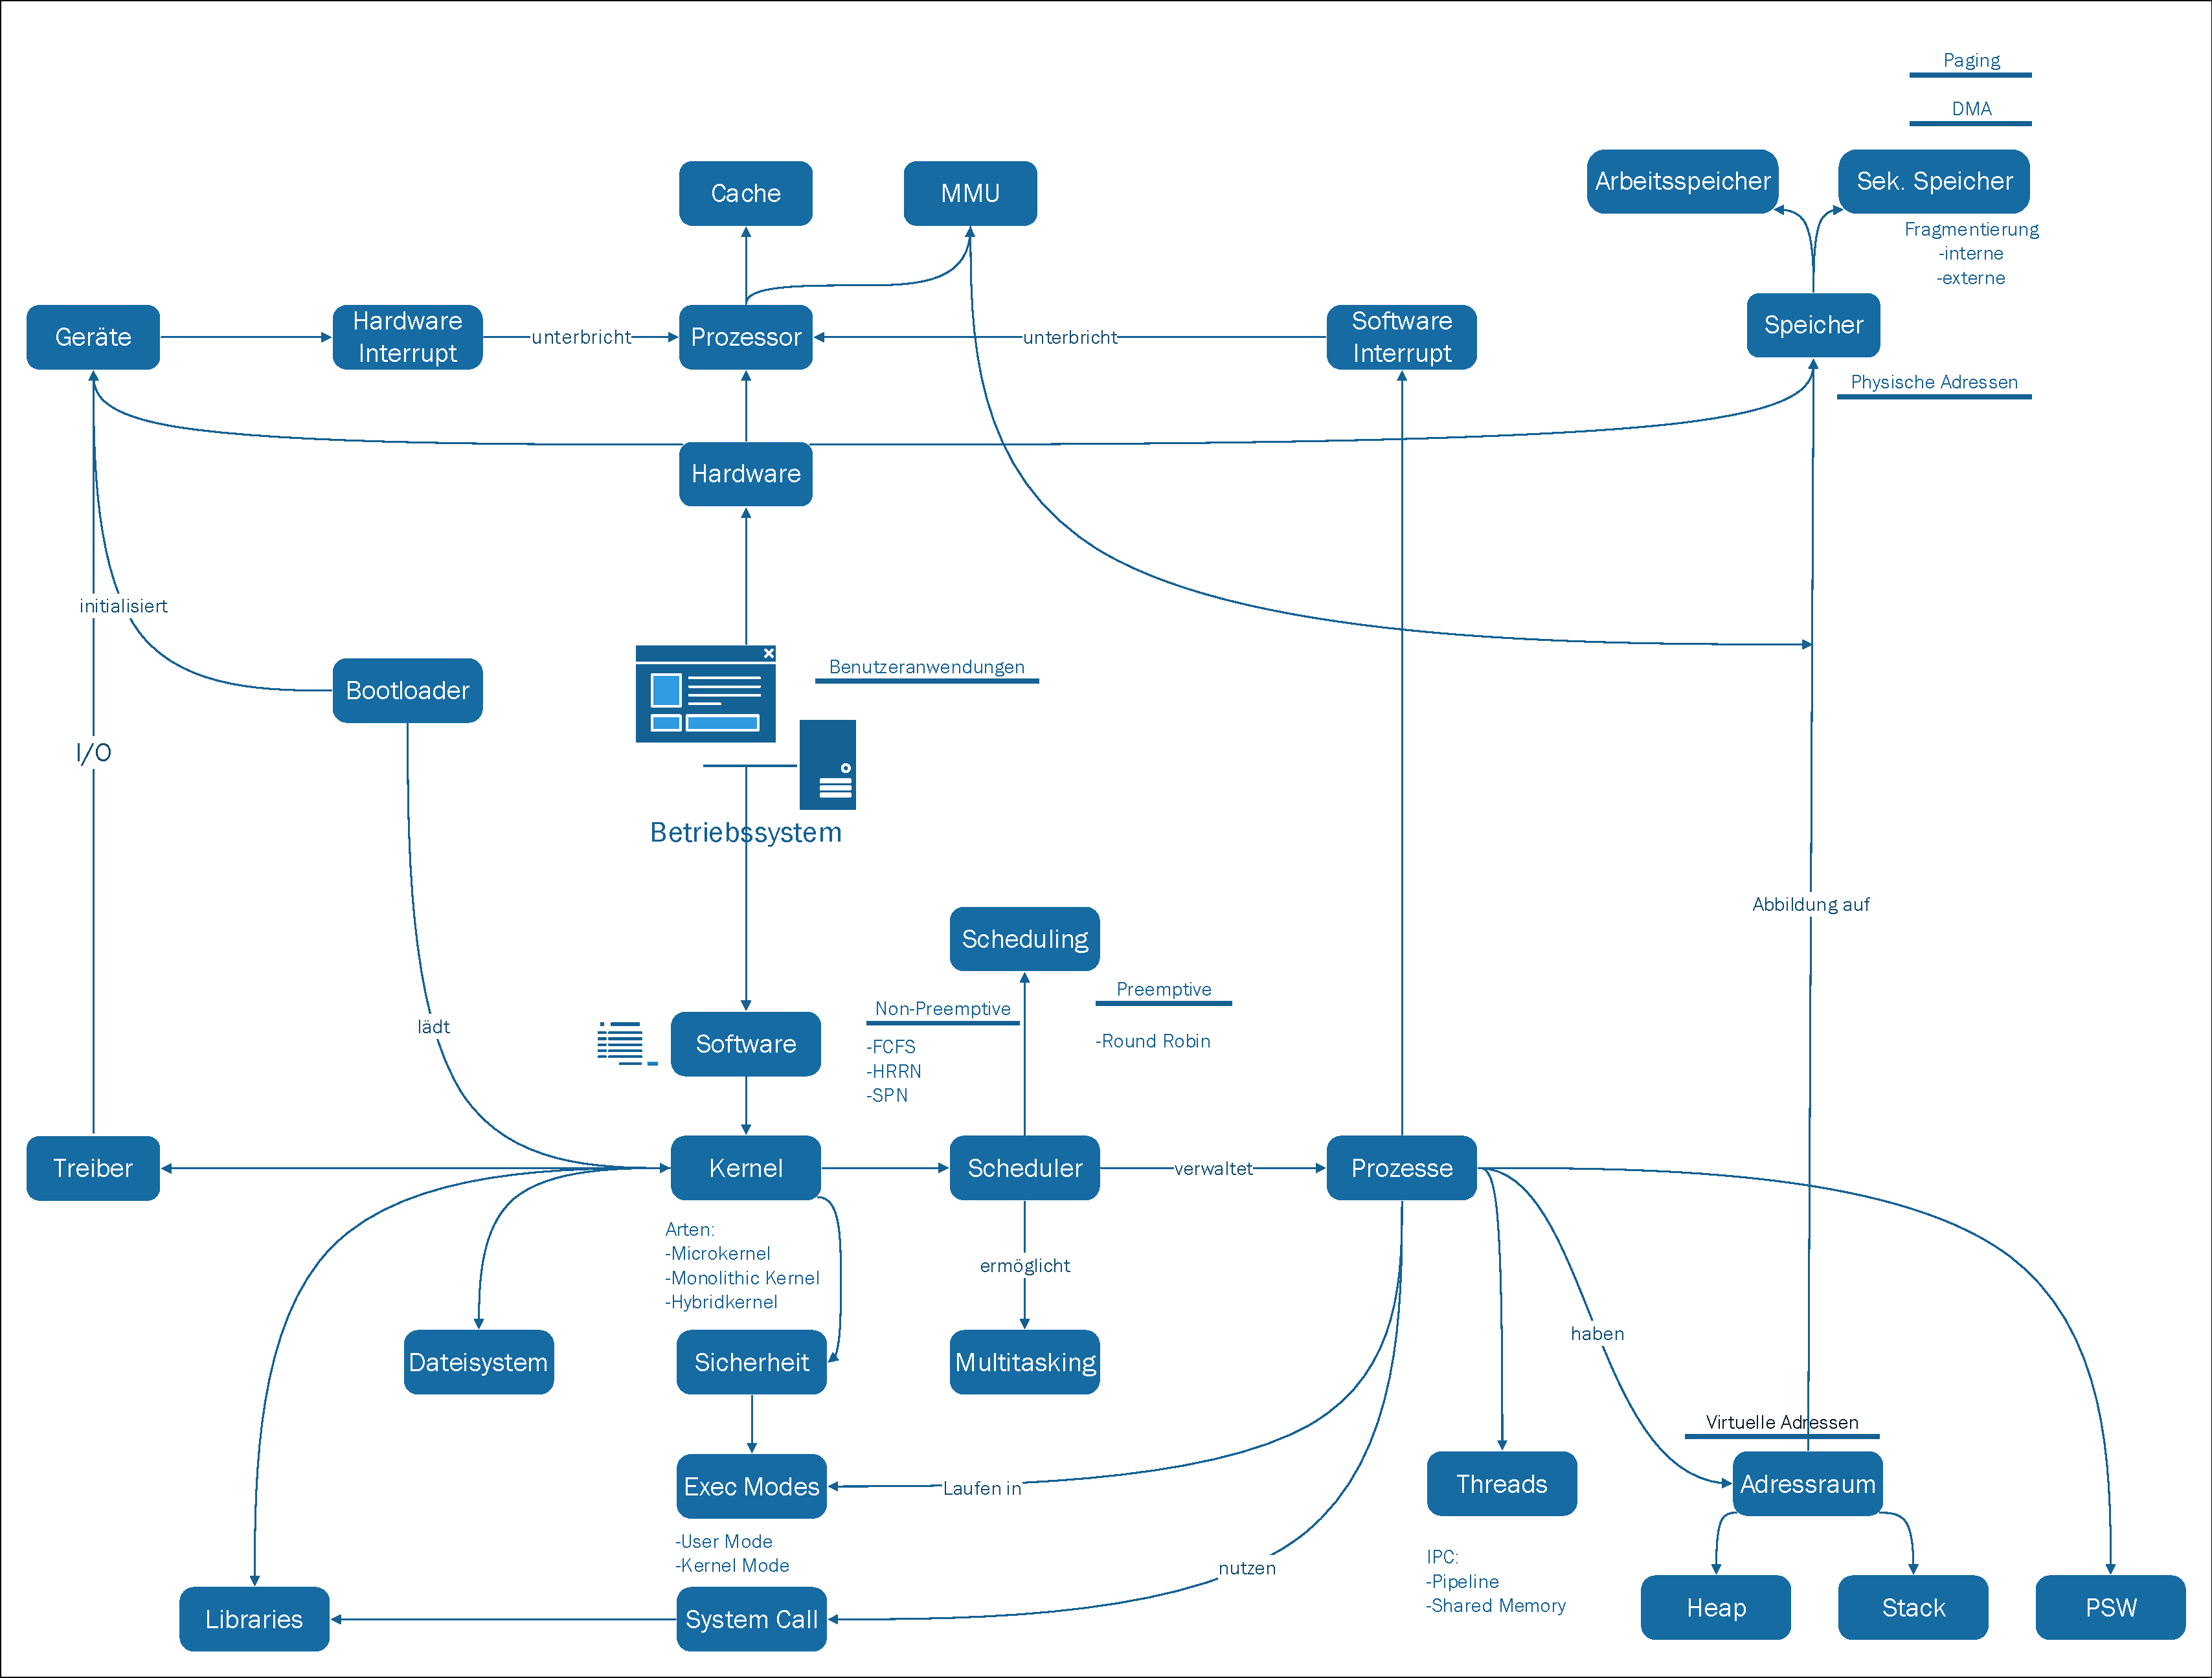
\includegraphics[width=\textwidth,page=1,trim={2 2 2 4},clip]{mindmap.pdf}



\end{document}
